% !TEX root = main.tex
% !TEX program = xelatex
\section{问题三的模型建立与求解}

\subsection{求解思路}

问题三在问题二的基础上增加了新的信息和新的代价：每天0:00先制定购电计划，
6:00、12:00和18:00还能获得新的光伏预报，并允许修改尚未执行的订单，但改单需要额外付费。

因此，\textbf{新预报更加准确，并不意味着一定要修改订单}。
如果预测变化较小，或者电池能够自行吸收偏差，修改订单反而可能增加费用。
本问需要同时考虑新光伏预报、当前储电量、普通购电及改单费用，以及5倍电价的紧急购电风险。

基于此，我们采用了\textbf{``预报修正--误差准备--滚动优化--实际执行''}的思路，在0:00、6:00、12:00和18:00分别重新判断未来购电方案。


\subsection{光伏预报修正与安全准备}

\subsubsection*{（1）融合官方预报与近期历史}

负载继续采用问题二的历史预测方法。光伏方面，附件3提供的是整点预报，而购电订单以10分钟为单位，因此先对同一版预报进行线性插值，将其转换为10分钟序列。

随后，将官方预报 $F_{r,t}$ 与近期同一时刻的实际光伏参考 $H_{r,t}$ 进行融合：

\begin{equation}
\widehat V_{r,t}
=
w_{r,g}F_{r,t}
+
(1-w_{r,g})H_{r,t}.
\end{equation}

其中，权重 $w_{r,g}$ 根据过去28天已经兑现的预测误差自动确定。官方预报近期更准确时，提高其权重；历史曲线更可靠时，则提高历史信息的作用。
该权重会随发布时间和预测提前量变化，并不是人为指定的固定比例。

\subsubsection*{（2）根据近期误差增加安全准备}

即使平均预测更加准确，也仍可能在个别关键时段低估供需缺口。由于少买的电可能需要按5倍价格紧急补购，因此需要在预测基础上保留一定安全余量。

定义过去某时段的净需求预测误差为

\begin{equation}
\varepsilon
=
\left[
(L-V)-(\widehat L-\widehat V)
\right]\Delta t.
\end{equation}

其中，$\varepsilon>0$ 表示实际缺电量大于预测值，即原计划低估了供需缺口。

我们使用过去28天已经发生的误差，将一天划分为8个3小时时段。
历史误差越接近当前时刻，权重越大，每向前一天权重乘以0.7；在每组误差中取加权0.60分位作为安全准备量。

我们的这种处理方法并不追求完全消除紧急购电，而是\textbf{在提前多购普通电与减少高价紧急购电之间进行权衡}。


\subsection{滚动购电与储能模型}

\subsubsection*{（1）决策变量与储能状态}

每个10分钟时段主要决策以下变量：

\begin{itemize}
    \item $q_t$：普通购电量；
    \item $x_t$：外网购电中用于储能充电的电量；
    \item $y_t$：光伏富余中用于储能充电的电量；
    \item $z_t$：储能设备向负载输出的电量；
    \item $e_t$：预计紧急购电量；
    \item $S_t$：时段结束后的电池内部储电量。
\end{itemize}

模型沿用前两问的供需平衡和储能结构。储电量满足

\begin{equation}
S_t
=
S_{t-1}
+
0.9(x_t+y_t)
-
\frac{z_t}{0.9},
\end{equation}

并满足

\begin{equation}
1200\leq S_t\leq10800.
\end{equation}

储能设备最大充、放电功率均为5000~kW，因此每10分钟最大充电量和放电量均为

\[
5000\times\frac{1}{6}
=
833.33\ \mathrm{kWh}.
\]

\subsubsection*{（2）购电调整费用}

设每天0:00制定的原始购电订单为 $q_t^0$，执行前最后一次调整后的订单为 $q_t^F$。

根据题目规定，增加订单的部分按原电价的1.5倍收费，减少订单的部分需承担50\%的违约费用。因此，最终普通购电及调整费用可统一写为

\begin{equation}
C_{\mathrm{ord}}
=
\sum_t
\left[
p_t q_t^F
+
\frac{1}{2}p_t
\left|
q_t^F-q_t^0
\right|
\right].
\end{equation}

多次修改同一个时段时，只比较最终订单与零点原订单的净变化，不重复计算中间修改产生的费用。

\subsubsection*{（3）优化目标}

滚动优化需要同时考虑普通购电费用、调整费用以及可能产生的紧急购电费用。因此，每次决策均以预计总费用最小为目标，即

\[
\min
\left(
\text{普通购电费用}
+
\text{调整费用}
+
\text{预计紧急购电费用}
\right).
\]

在给定预测信息后，目标函数与供需平衡、储能状态、容量和功率限制均为线性关系，因此采用线性规划进行求解。


\subsection{日内滚动求解过程}

每天按照以下顺序进行滚动决策：

\begin{enumerate}
    \item \textbf{0:00：}根据当前历史信息、0:00光伏预报和真实储电量制定当天原始购电计划；
    \item \textbf{6:00：}读取新的光伏预报和此时真实储电量，仅重新安排6:00以后尚未执行的订单；
    \item \textbf{12:00和18:00：}重复上述过程，已经执行的订单保持不变；
    \item \textbf{实际运行：}按照真实负载和光伏供电。当普通购电不足时，优先由储能补充，储能仍无法满足时再进行紧急购电；
    \item \textbf{跨日衔接：}24:00的剩余储电量直接作为下一天的初始储电量。
\end{enumerate}

2025年2月1日至12月31日共334天，每天进行4次优化，共完成1336次滚动线性规划。


\subsection{方案比较与最终结果}

为了确定最终策略，在相同负载预测、设备参数和结算规则下，对不同光伏处理方法及风险准备方法进行比较，结果见表~\ref{tab:q3_compare}。

\begin{table}[htbp]
\centering
\caption{问题三不同方案的全年费用比较}
\label{tab:q3_compare}
\begin{tabular}{lccc}
\hline
方案 & 普通结算/万元 & 紧急购电/万元 & 总费用/万元 \\
\hline
直接使用官方预报 & 1289.96 & 127.56 & 1417.51 \\
历史误差融合预报 & 1276.36 & 132.51 & 1408.87 \\
提升树修正预报 & 1279.46 & 136.80 & 1416.26 \\
融合预报+近期误差准备 & \textbf{1294.35} & \textbf{20.31} & \textbf{1314.65} \\
\hline
\end{tabular}
\end{table}

可以看出，仅提高预测精度并不能保证最低费用。历史融合方案虽然普通购电费用较低，但仍会在部分关键时段低估供需缺口，从而产生较多紧急购电。

加入近期误差准备后，普通结算增加约17.98万元，但紧急购电费用减少约112.20万元，总费用减少约94.22万元。因此，本文最终采用

\[
\boxed{
\text{历史融合预报}
+
\text{近期误差准备}
+
\text{滚动线性规划}
}
\]

作为问题三的购电策略。

最终334天的普通结算费用为

\[
12943484.52\ \mathrm{元},
\]

紧急购电费用为

\[
203050.97\ \mathrm{元},
\]

总费用为

\[
\boxed{13146535.49\ \mathrm{元}}.
\]

全年共有164天出现紧急购电。

\subsubsection*{月度费用分析}

如图~\ref{fig:q3_monthly}所示，2月至12月各月相对于初始融合方案均实现费用下降。节省的主要来源不是减少普通购电，而是通过适量提前准备，减少5倍价格的紧急购电。

但月度节省并不意味着每天费用都下降。全年共有250天费用减少、59天费用增加、25天基本不变。同时仍存在部分未被实际接收的普通订单，说明风险准备本身也需要付出一定成本。

\begin{figure}[H]
    \centering
    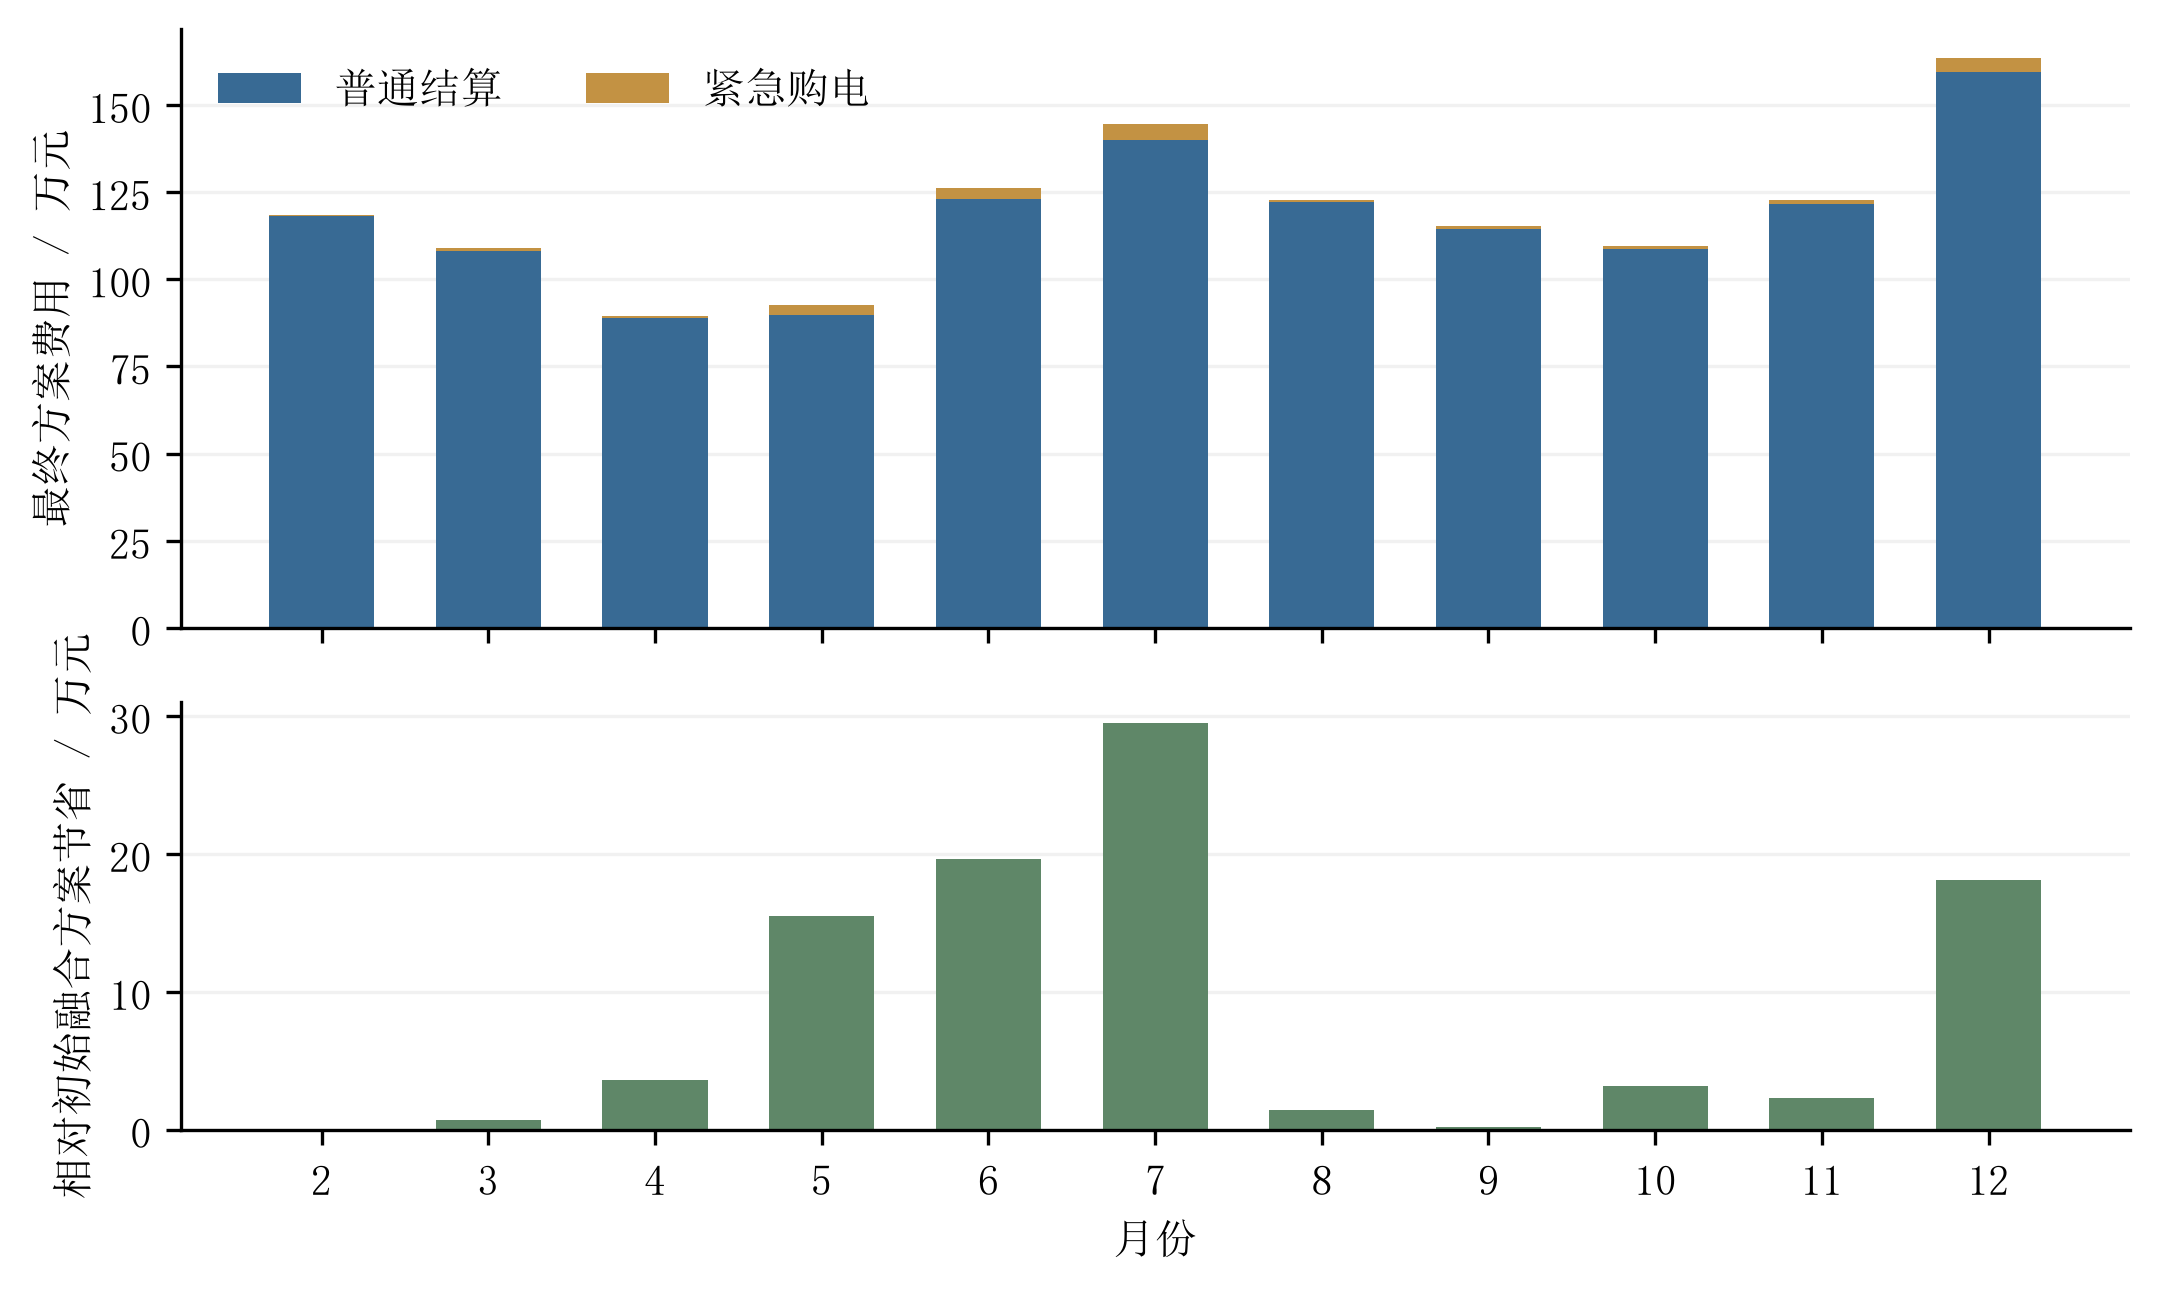
\includegraphics[width=0.9\textwidth]{fig/final_monthly.png}
    \caption{最终方案的月度费用及相对初始融合方案的节省}
    \label{fig:q3_monthly}
\end{figure}


\subsection{指定日期运行分析}


相应的紧急购电情况见表~\ref{tab:q3_emergency}。

\begin{table}[H]
\centering
\caption{表2 指定日期零点原计划的部分时段购电量（kWh）}
\label{tab:q3_emergency}
\begin{tabular}{|c|c|c|c|c|c|c|c|}
\hline
\multicolumn{2}{|c|}{2025.3.20} & \multicolumn{2}{c|}{2025.6.21} & \multicolumn{2}{c|}{2025.9.23} & \multicolumn{2}{c|}{2025.12.21} \\
\hline
时间段 & 购电量 & 时间段 & 购电量 & 时间段 & 购电量 & 时间段 & 购电量 \\
\hline
10:00--10:10 & 0.00 & 10:00--10:10 & 0.00 & 10:00--10:10 & 0.00 & 10:00--10:10 & 0.00 \\
\hline
12:00--12:10 & 586.14 & 12:00--12:10 & 0.00 & 12:00--12:10 & 436.19 & 12:00--12:10 & 948.82 \\
\hline
14:00--14:10 & 0.00 & 14:00--14:10 & 0.00 & 14:00--14:10 & 0.00 & 14:00--14:10 & 0.00 \\
\hline
16:00--16:10 & 489.39 & 16:00--16:10 & 110.71 & 16:00--16:10 & 472.88 & 16:00--16:10 & 806.52 \\
\hline
18:00--18:10 & 716.29 & 18:00--18:10 & 432.73 & 18:00--18:10 & 827.44 & 18:00--18:10 & 731.68 \\
\hline
20:00--20:10 & 0.00 & 20:00--20:10 & 0.00 & 20:00--20:10 & 5.90 & 20:00--20:10 & 0.00 \\
\hline
\end{tabular}
\end{table}

题目指定日期的零点原计划、最终普通订单及全天费用见表~\ref{tab:q3_days}。

\begin{table}[H]
\centering
\caption{问题三指定日期的全天购电及费用结果}
\label{tab:q3_days}
\begin{tabular}{ccccc}
\hline
日期 &
零点原计划/kWh &
最终普通订单/kWh &
紧急购电/kWh &
总费用/元 \\
\hline
3月20日  & 64012.35 & 62868.01 & 95.59 & 40254.40 \\
6月21日  & 39766.06 & 39547.19 & 14.64 & 21874.93 \\
9月23日  & 68933.65 & 69071.70 & 6.38 & 43652.00 \\
12月21日 & 94785.86 & 95867.85 & 45.47 & 62318.84 \\
\hline
\end{tabular}
\end{table}

四个指定日期均出现了少量紧急购电，其中3月20日的紧急购电量最大，
发生在20:40--20:50；9月23日仅在20:30--20:40补购6.38~kWh。
12月21日虽然出现两次紧急购电，但单次电量均较小。

结合图\ref{fig:q3_days}可以看到，大多数普通订单后的供电缺口均可由储能设备补充。

例如，3月20日晚间电池已接近1200~kWh的储电下限，因此仍有95.59~kWh的缺口无法通过储能满足，只能进行紧急购电；9月23日仅出现6.38~kWh紧急购电。

这说明，是否发生紧急购电不仅取决于全天总电量是否充足，还取决于缺口出现的具体时刻以及当时的储电状态。

\begin{figure}[H]
    \centering
    \includegraphics[width=0.95\textwidth]{fig/q3_specified_days.png}
    \caption{典型日期的供需、储电状态与缺口补充过程}
    \label{fig:q3_days}
\end{figure}


\subsection{日内新预报的实际费用价值}

为了单独判断6:00、12:00和18:00新光伏预报的价值，本文设置三个逐步增加信息的对照方案，结果见表~\ref{tab:q3_info_value}。

\begin{table}[H]
\centering
\caption{日内反馈与新光伏预报的费用价值}
\label{tab:q3_info_value}
\begin{tabular}{lc}
\hline
条件 & 总费用/万元 \\
\hline
零点订电，全天不调整 & 1614.80 \\
允许日内反馈和改单，但不使用新预报 & 1439.29 \\
允许日内反馈和改单，并使用新预报 & 1417.51 \\
\hline
\end{tabular}
\end{table}

结合图~\ref{fig:q3_information}可见，允许根据日内实际运行情况重新调整订单后，总费用首先减少175.51万元；在此基础上进一步使用6:00、12:00和18:00的新官方预报，又减少21.78万元。

因此，197.28万元不能全部解释为新光伏预报带来的收益。更准确地说，\textbf{日内滚动调整本身带来主要收益，而新的官方光伏预报在此基础上进一步改善了购电决策。}

\begin{figure}[H]
    \centering
    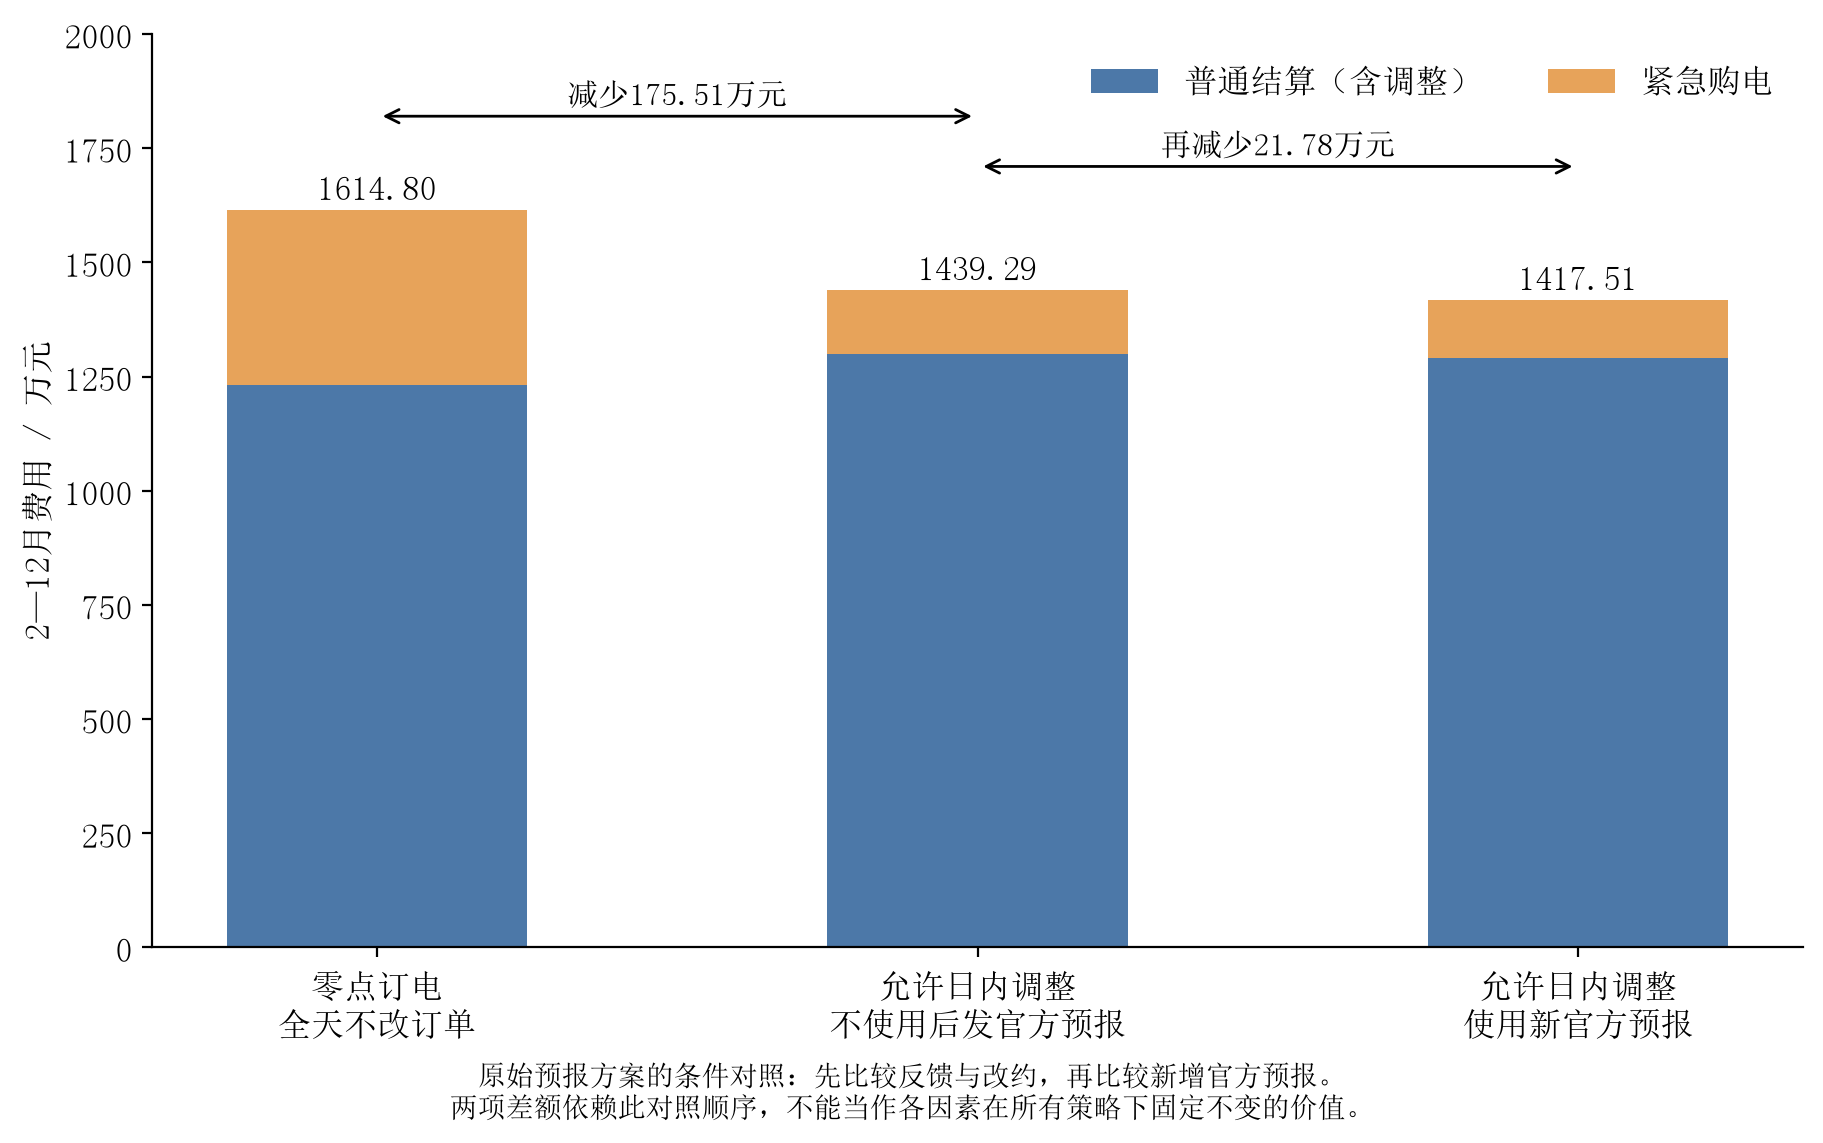
\includegraphics[width=0.85\textwidth]{fig/information_value.png}
    \caption{日内反馈、订单调整与新增官方预报的费用价值}
    \label{fig:q3_information}
\end{figure}


\subsection{参数检验与模型可信度}

模型中的风险准备需要确定误差分位、时间衰减、误差分组和历史窗口。为避免参数选择过于主观，本文对这些参数进行灵敏度比较，结果如图~\ref{fig:q3_parameter}所示。

\begin{itemize}
    \item \textbf{误差分位：}在0.55--0.80范围内，0.60对应的总费用最低；
    \item \textbf{时间衰减：}取0.7时费用低于0.8和1.0，说明近期误差应具有更高权重；
    \item \textbf{误差分组：}在1、2、3、4和6小时分组中，3小时方案费用最低；
    \item \textbf{历史窗口：}14、28和56天的费用差异很小，因此采用能够覆盖4个完整星期的28天。
\end{itemize}

\begin{figure}[H]
    \centering
    \includegraphics[width=0.95\textwidth]{fig/parameter_interpretability.png}
    \caption{近期误差准备参数的费用依据}
    \label{fig:q3_parameter}
\end{figure}

上述参数均来自相同模型条件下的实际费用比较，而非人为指定。进一步对保存的订单、储电状态、功率限制和逐时供需进行复核，结果均满足模型约束。

需要说明的是，这些参数是在2025年数据条件下选出的，能够支持本题范围内的模型选择，但不能据此认为在其他年份或其他微网中仍保持相同的最优取值。